\documentclass[12pt]{article}
\usepackage{pictex,amsmath,amsthm,amssymb}
\usepackage{amsbsy,fullpage,fancyhdr,verbatim}
\usepackage{graphics,graphicx}

\setlength{\voffset}{-0.25in}
\setlength{\headsep}{+0.5in}
\setlength{\parskip}{1em}
\setlength{\parindent}{0em}

\begin{document}
\begin{enumerate}
	%1
	\item Draw logic circuit corresponding to the follow Boolean expressions:
	\begin{itemize}
		\item z = $\overline{(A+B+\overline{C}D \overline{E})} + \overline{B}C \overline{D}$
		\item x = $MN(P + \overline{N})$
	\end{itemize}
	%2
	\item Simplify the following expressions using DeMorgan 's theorem:
	\begin{itemize}
		\item X = $\overline{A \overline{(B + \overline{C})}D}$
		\item Y = $\overline{\overline{\overline{AB}C}D}$
	\end{itemize}
	%3
	\item Simplify the following expressions:
	\begin{itemize}
		\item X = $\overline{A}$BCD + A $\overline{B}$ $\overline{C}$ $\overline{D}$ + A $\overline{B}$ $\overline{(\overline{C} + D)}$ + A $\overline{(B + C)}$D + A $\overline{(B + \overline{C} + \overline{D}}$ + B $\overline{C})$ + ABC
		\item Y = $\overline{A}$C $\overline{D}$ + A $\overline{B}$ $\overline{C}$ + $\overline{(C + D)}$ + $\overline{A}$ $\overline{B}$CD + $\overline{(\overline{A} + \overline{C})} \overline{D}$
	\end{itemize}
	%4
	\item Exercise 10: Transform the following circuits using only NAND gates:
	\begin{itemize}
		\item a)\\
		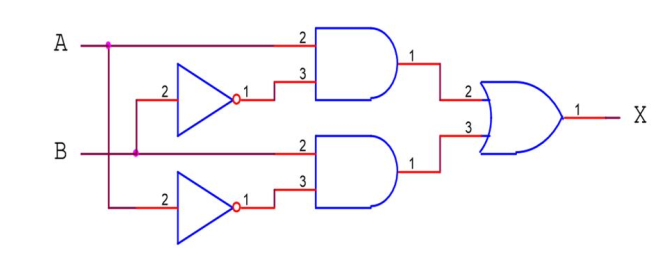
\includegraphics[scale = 1.05]{hinh.png}\\
		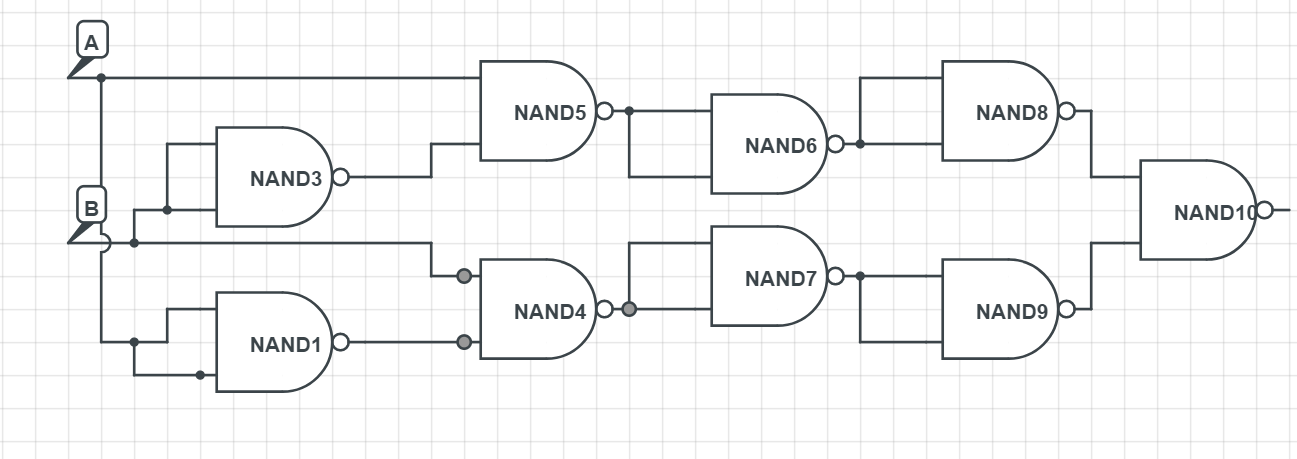
\includegraphics[scale = 0.65]{Bai10a.png}
	\bigbreak
		\item b) \\
		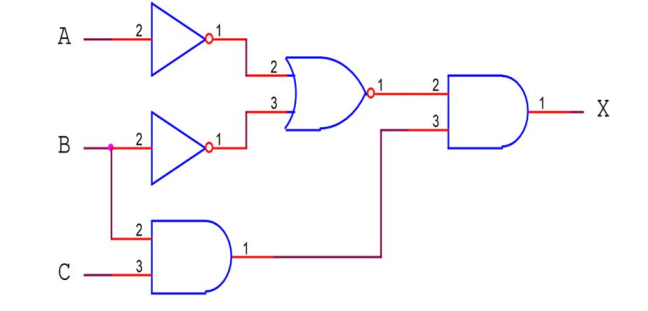
\includegraphics[scale = 1.05]{hinh1.png} \\
		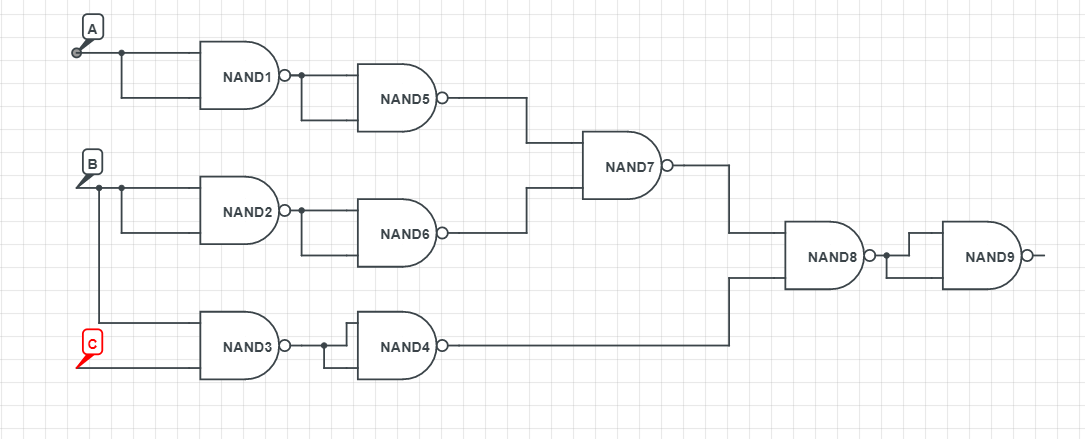
\includegraphics[scale = 0.75]{Bai10b}
	\end{itemize}
	%5
	\item Exercise 11: Transform the following circuits using only NOR gates:
	\begin{itemize}
		\item a) \\
		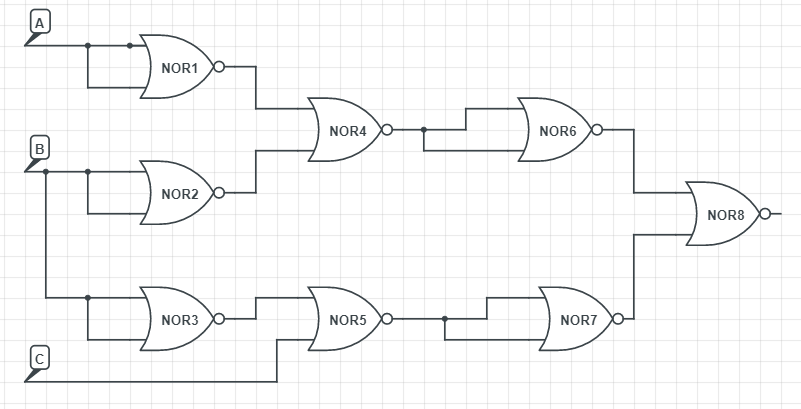
\includegraphics[scale = 0.75]{Bai11a.png}
		\item b) \\
		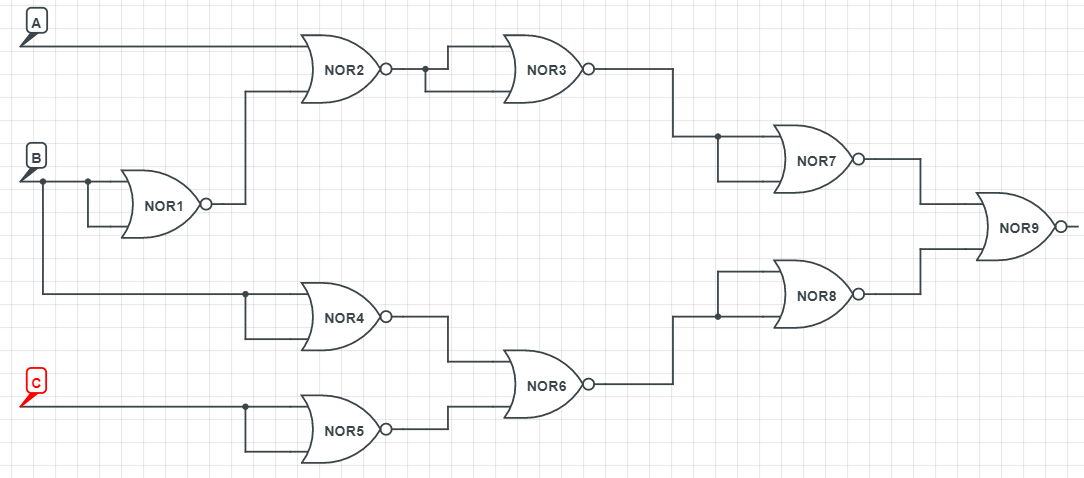
\includegraphics[scale = 0.75]{Bai12b.png}
	\end{itemize}
	%6
	\item Exercise 12:Build a 2-input NAND gate using only 2-input NOR gates:\\
	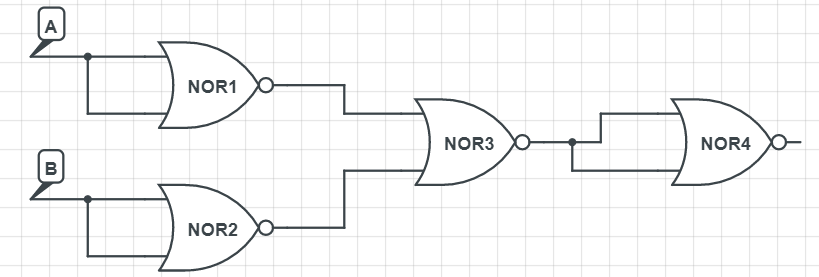
\includegraphics[scale = 0.75]{Bai12a.png}
	\item Exercise 13:Build a 2-input NOR gate using only 2-input NAND gates:\\
	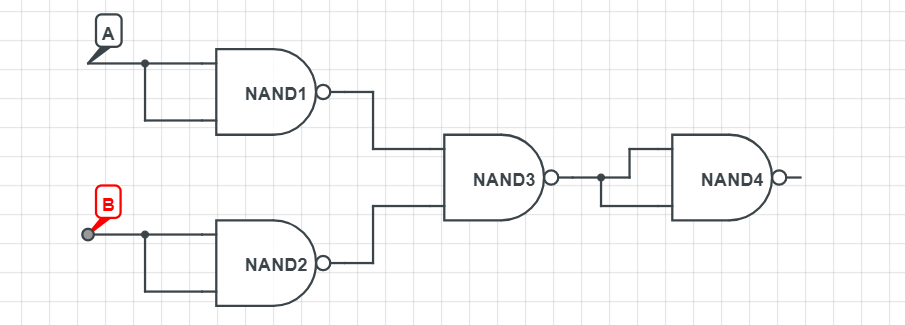
\includegraphics[scale = 0.75]{Bai13.png}
\end{enumerate}
\end{document}
